\section{The structure}

Mezzanine Floor Racking Systems are modular structures which consist of beams, columns and joists, as shown on Figure \ref{mezzanine}.

\begin{figure}[h!]
\centering
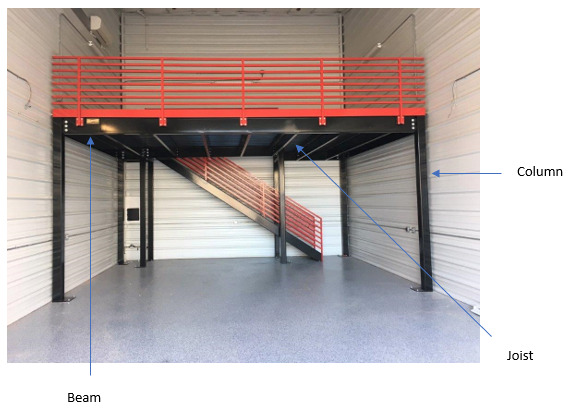
\includegraphics[width=\textwidth]{Images/General/mz.jpg}
\caption{Mezzanine parts. \vspace{0.5cm} Source: http://www.firststorage.co.za}
\label{mezzanine}
\end{figure}

\vspace{-0.7cm}

The resistance of a structural member rely on the material, geometry of the section and the length of the member. By default, the framework is programmed to work with steel ASTM A1011 SS Grade 36/2, which has the properties shown on Table \ref{properties}.

\begin{table}[h!]
\centering
\begin{adjustbox}{max width=\textwidth}
\begin{tabular}{c c}
\hline
\textbf{Parameter} & \textbf{Value} \\ \hline
Density $\left[kg/m^3\right]$ & 7850 \\ \hline
Young Modulus $[GPa]$ & 200 \\ \hline
Coefficient of Poisson & 0.3 \\ \hline
Yield strength $[MPa]$ & 248.25 \\ \hline
Ultimate strength $[Mpa]$ & 440 \\ \hline
\end{tabular}
\end{adjustbox}
\caption{Strength properties.}
\label{properties}
\end{table}

Other materials can be defined and selected by the user, even composite cross sections can be implemented.
 
 


